\chapter{Methodology}

This chapter will chronologically outline the steps planned and taken in the progression of the project.

The next chapter, Experiment Design, will detail how this methodology has been implemented.

At the start of the project, a high-level representation of the research and development steps required to complete the project was created as a Gannt chart. These steps were allocated a time frame and a sprint was planned at the start of each time frame.

This workflow is best described as a modified scrum methodology with a variable and flexible sprint window for each objective. Adherence to agile principles has guided decision-making when multiple options were available.

While each sprint was different, sprints broadly involved defining a clear goal and pursuing it until the end of the sprint window. While the sprint windows were not strict cut-offs, the primary focus of my time would change upon the start of a new sprint window.

The steps detailed in this chapter deviate from the initial plan specified in the Gannt chart. The changing project plan is inline with agile principles, embracing changing requirements and changing the plan as deemed necessary during reflection between sprints.

\section{Research Potential Projects}

The first step in this project was to identify potential project ideas. This was done with brainstorming, both by thinking about the project and talking about it with others.

The project ideas broadly fell into two categories, engineering, where the objective is to produce an application, and research, where the objective is to provide insight or an answer to an unknown.

A personal goal for me in this project was to develop my skills in machine learning and artificial intelligence. Evaluating the iArsenic models and producing alternative models with machine learning appealed to me as the most exciting project available. Because the project already contained a wealth of existing work, the objectives of this dissertation could build off this work instead of starting from scratch. This enabled higher level and higher impact objectives to be set. 

As Dr Mohammed Hoque agreed to be the client to this project I was able to commit to this project, confident in knowing it had purpose and direction from the client.

\section{Continuously Identifying Client Requirements}

In line with agile principles, the priority of this project was to satisfy the clients requirements. Therefore regular communications with Dr Hoque were prioritised in the form of emails and video calls where I would provide progress updates and Dr Hoque would provide feedback and direction. 

\subsection{Clarifying the Project Objectives}

Originally the vision of the project was to develop machine learning based models and compare their performance to the existing iArsenic models.

This initial vision is however does not define several key aspects of the project. How does one evaluate the performance of an iArsenic model? How does this compare to an evaluation of a machine learning based model? What is the purpose of developing new models and comparing them to the existing ones?

Ultimately the desired outcomes were clearly defined as the following:

\textbf{Desired Outcomes}

\begin{enumerate}
  \label{desired_outcomes}
  \item To evaluate the existing models
  \item To compare the performance of the existing models with typical machine-learning-based models
\end{enumerate}

Desired Outcome 1 was requested from the client. Evaluating the models informs the client of how each iteration of the models has impacted their performance and, because this model is deployed, verifies the quality of the predictions being made in deployment.  While the existing models were developed with expert knowledge, prior to the evaluations conducted in this project the performance of the iArsenic models was unknown.

The purpose of desired outcome 2 builds from the assertion made in \cite{Fleming2021} that machine learning should be part of Earth and Environmental Science. iArsenic provided an opportunity for a case study where expert system models can be compared to supervised learning models. 

\section{Research Applied Machine Learning Methodologies}

To design implement and evaluate machine learning models for iArsenic, I first had to research machine learning to understand what specific areas in machine learning could be applied to this dataset to achieve the desired outcomes of the project and then had to develop these models in code to gain the practical experience required.

Chapter 2 of \cite{Aurélien2017}, Hands-On Machine Learning with Scikit-Learn and TensorFlow, was the primary resource for breaking through the barrier of theoretical knowledge, gained from written sources such as \cite{Caruana2006} which compares several supervised machine learning models in different applications, to actually producing my own implementations of these models.

% TODO, could all the code in this section be moved to experiment design
\section{Understanding the iArsenic Code}

The iArsenic code provided the following key functions:

\begin{enumerate}
  \label{ia_functions}
  \item Producing a standard dataset
  \item Generating iArsenic models from a dataset
  \item Generating predictions from these generated models
\end{enumerate}

To learn how to achieve this functionality, I would read the iArsenic code in GitHub and experiment with it as an npm package.

\subsection{Producing a standard dataset}

The iArsenic script csv-to-json.js makes exporting a standardised dataset trivial.

This function is implemented in the project via an package script:

\begin{figure}[ht]
\begin{minted}[linenos, breaklines]{json}
"scripts": {
    "load-src-data": "mkdir well_data ; node node_modules/preprocessing/preprocessing/cli/csv-to-json.js -p node_modules/preprocessing/data/*.csv -o well_data/src_data.json",
\end{minted}
\label{fig:x load_ia_data}
\caption{Package.json snippet showing script to load data from iArsenic}
\end{figure}

\subsection{Generating iArsenic models from a dataset}

To verify that a model can generalise to new cases, it must be trained on a subset of the data and tested on a separate subset of data which it has not been previously exposed to, see \ref{eval} on page \pageref{eval}. In the iArsenic web application, the models are trained on the entire source dataset. See \ref{fig:x imp_iam_webapp} on page \pageref{fig:x imp_iam_webapp} for a flowchart showing this implementation.

Generating the iArsenic models from a training subset of the data was done by passing 4 of the 5 subsets of the data to the iArsenic model generator. This was done for each of the 5 subsets of the data for each of the 3 iArsenic models. See \ref{fig:x programmatically_gen_ia_model} on \pageref{fig:x programmatically_gen_ia_model} to see the code that achieved this.

\begin{figure}[ht]
    \centering
    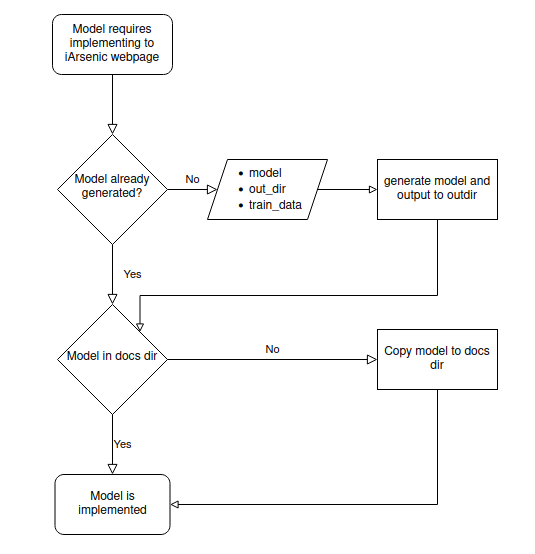
\includegraphics[scale=0.6]{figures/implement_ia_model_to_webapp.png} 
    \caption{Flowchart showing process to implement model in iArsenic webapp}
    \label{fig:x imp_iam_webapp}
    \small The code that generates the models can be found at: \url{https://github.com/portsoc/iArsenic/blob/master/preprocessing/cli/produce-aggregate-data-files.js}
\end{figure}

\begin{figure}[h]
    \begin{minted}[linenos, breaklines]{python3}
def gen_model(train_src, out_dir, model):
  if not os.path.exists(out_dir):
    os.mkdir(os.path.join(out_dir))

  cmd = [
    'node',
    'node_modules/preprocessing/preprocessing/ cli/produce-aggregate-data-files.js', 
    '-m',
    model,
    '-o',
    out_dir,
    '-p',
    train_src,
    'node_modules/preprocessing/data/mouza-names.csv',
  ]
  stdout = check_output(cmd).
    decode(sys.stdout.encoding).
    replace('\n', '')
    
  print(stdout)
    \end{minted}
    \caption{Python code used to programmatically generate iArsenic models. In iArsenic this is done via the command line}
    \label{fig:x programmatically_gen_ia_model}
    \small The file containing this code can be found at: \url{https://github.com/JavaRip/UoP-SoftEng-Dissertation/blob/main/models/model_utils/gen_ia_model.py#L9-L25}
\end{figure}

\subsection{Generating predictions from generated iArsenic models}

The web application index.html file shows a script.js file is used, in this file a global function called produceEstimate is called from the estimator.js script. See \ref{fig:x produce_estimate_call} on \pageref{fig:x produce_estimate_call} to see this function call.

\begin{figure}
    \begin{minted}[linenos, breaklines]{python3}
    const estimate = produceEstimate(aggregateData, inputs.division, inputs.district,
      inputs.upazila, inputs.union, inputs.mouza, inputs.depth, inputs.colour, inputs.utensil, inputs.flooding);
    \end{minted}
    \caption{Code used in iArsenic to produce estimate from a model in the webapp}
    \label{fig:x produce_estimate_call}
    \small The file containing this code can be found at: \url{https://github.com/portsoc/iArsenic/blob/master/docs/script.js#L340-L341}
\end{figure}

\section{Developing New Models}

To familiarise myself with implementing machine learning models, I initially followed the tutorial in Chapter 2 of \cite{Aurélien2017}'s book Hands-On Machine Learning with Scikit-Learn. I then implemented 4 separate supervised learning models on 25 datasets from the internet, see \ref{fig:x 4_m_25_d}. This was to develop my skills, in line with the agile principle continuous attention to technical excellence.

\begin{landscape}
    \begin{figure}[ht]
        \centering
        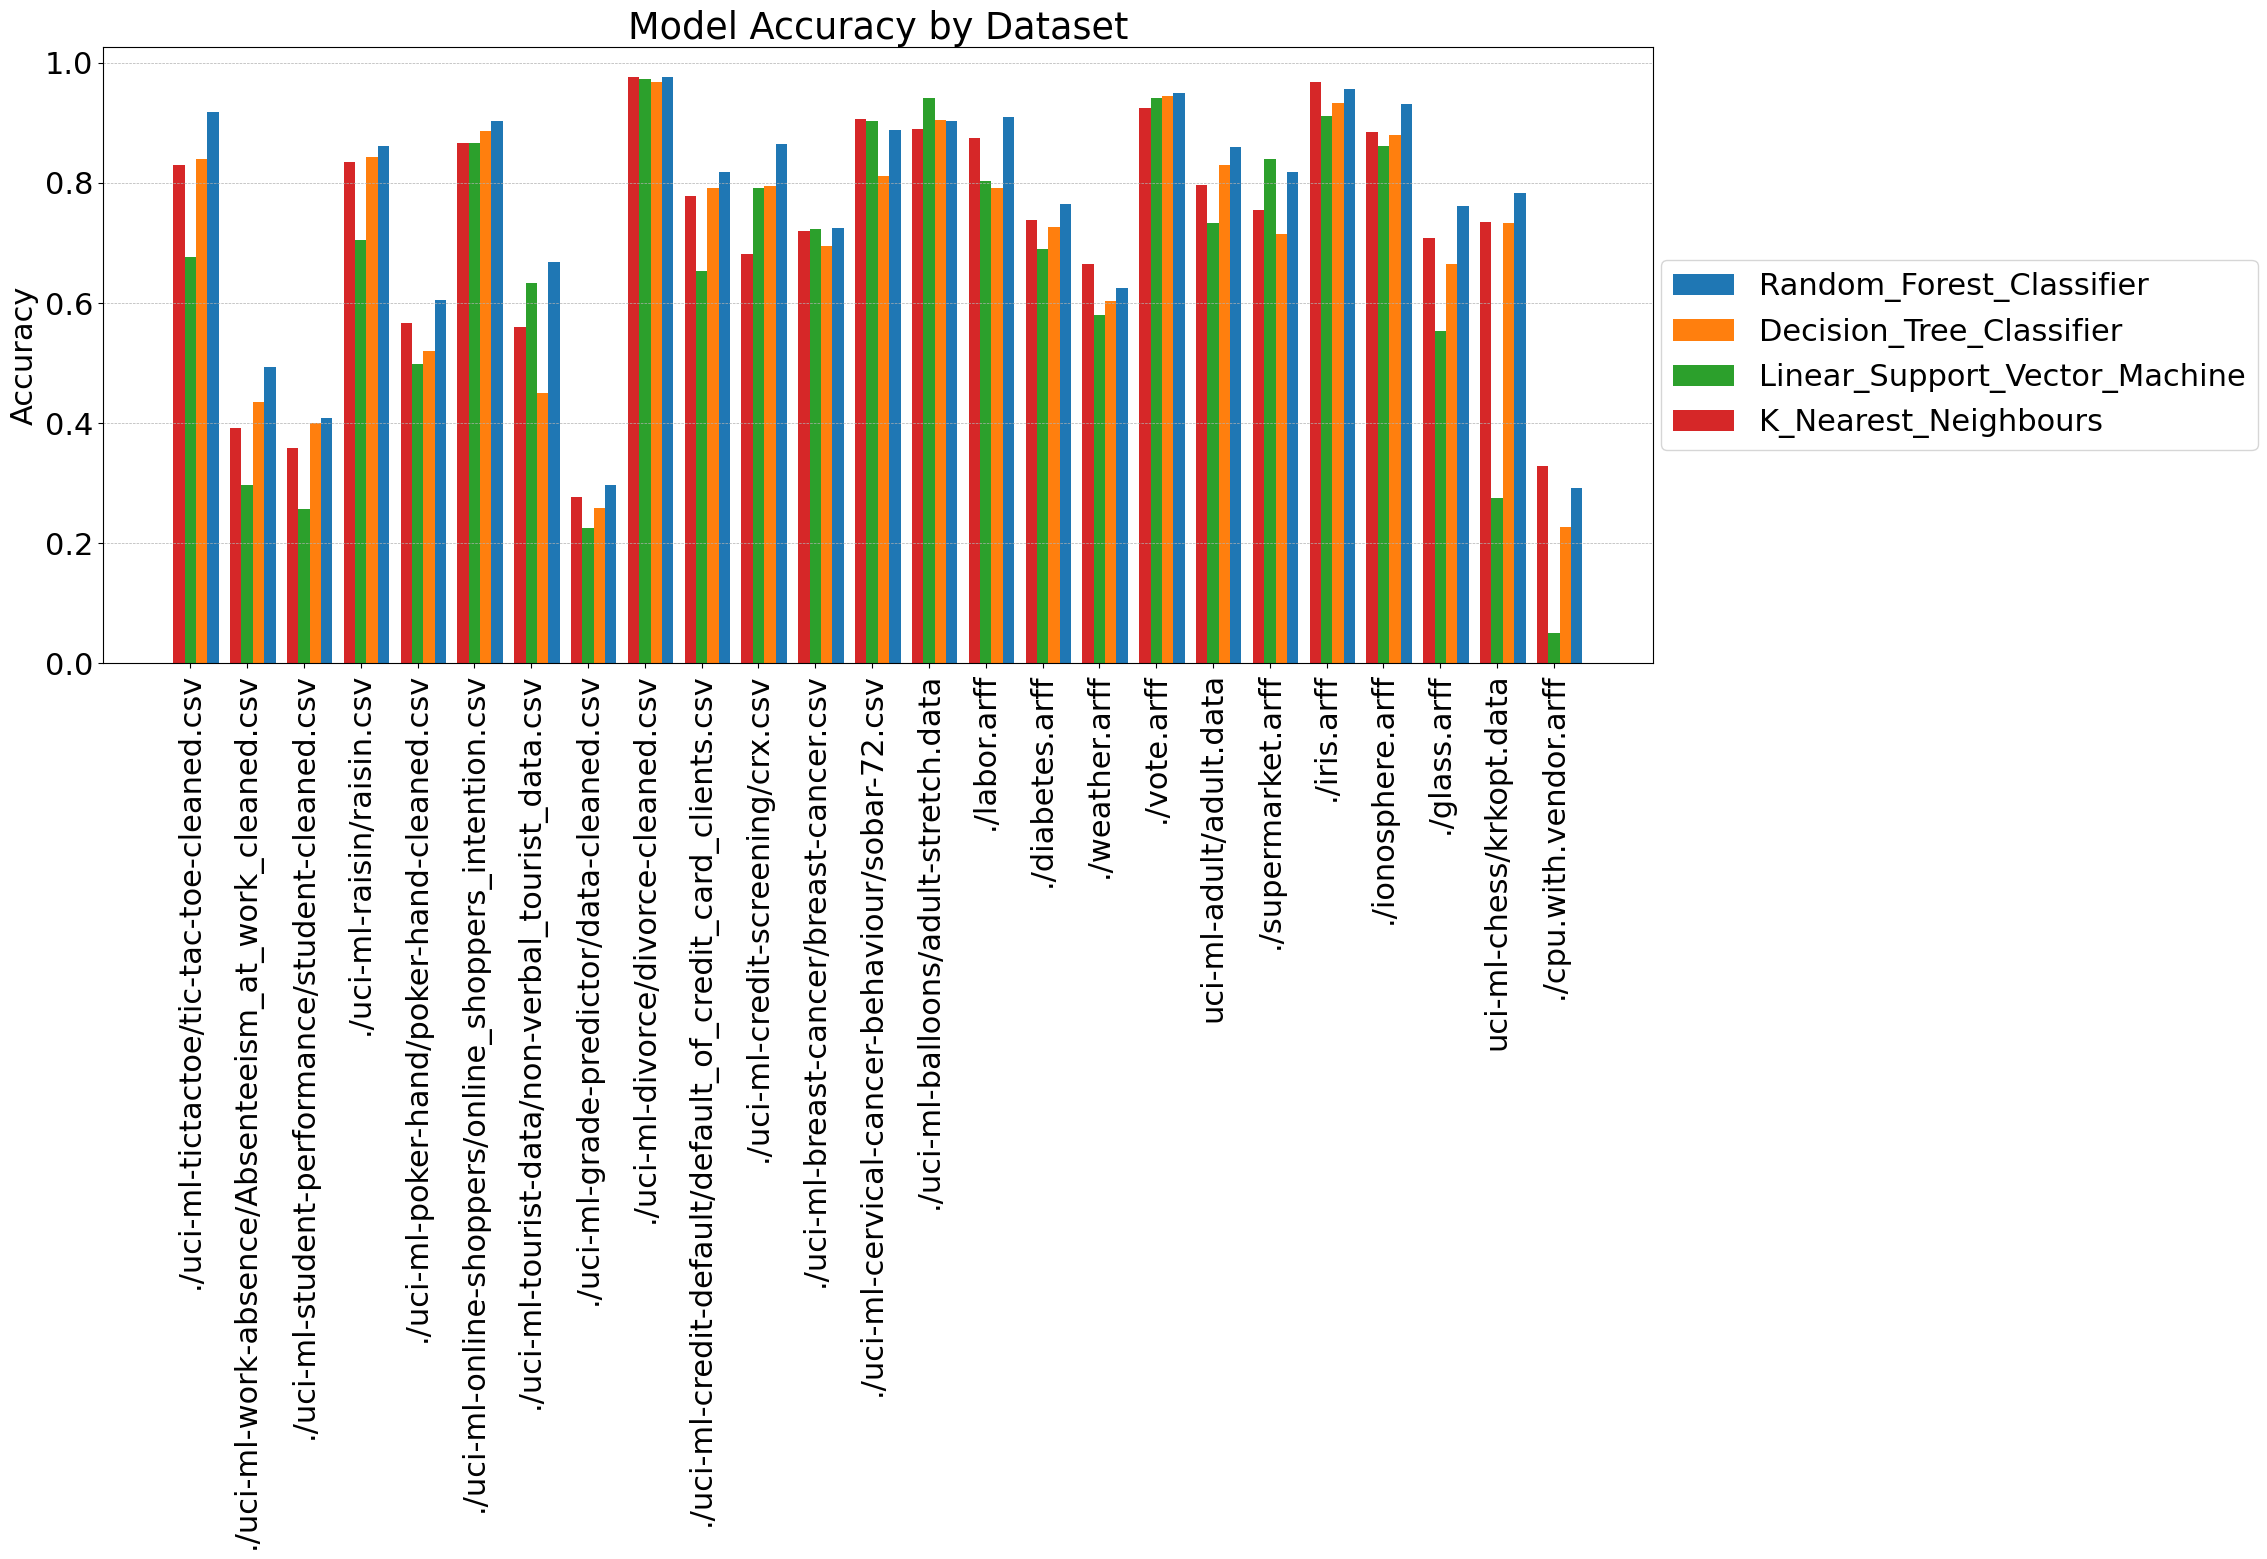
\includegraphics[scale=0.375]{figures/4_models_25_datasets.png} 
        \caption{Summary of results of supervised model implementation practice}
        \label{fig:x 4_m_25_d}
    \end{figure}
\end{landscape}

\section{Integrating iArsenic and scikit-learn}

The prototype implementations of both iArsenic and machine learning based models allowed each model to take input data and produce estimations individually. 

Because it takes multiple days to run every experiment required, it is not practical to have a human run each model individually. The time between an experiment finishing and the next starting will depend on when the human gets around to it. By making the models run programmatically this is not an issue. It also makes the project to be more portable, allowing it to be run on a remote server or high performance computer.

To run both NodeJS based iArsenic models and Python based scikit-learn models an integration layer between Python and NodeJS had to be created. Python was chosen as the main program to run the NodeJS code from as a personal preference. Using NodeJS would also have been a reasonable choice. See \ref{fig:x ia_model_sd} on page \pageref{fig:x ia_model_sd} to see the flow of data from the main.py script to the iArsenic models to produce estimates for a test dataset.

\begin{figure}
    \centering
    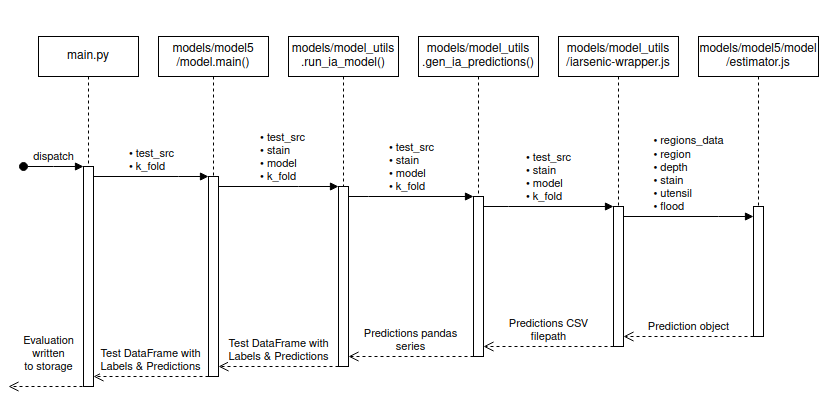
\includegraphics[width=\textwidth]{figures/ia_model_sd.png} 
    \caption{Sequence diagram showing Python to NodeJS variable bridge over storage}
    \label{fig:x ia_model_sd}
\end{figure}

\section{Main Project Structure}

The project architecture has a top-level main file, which when run will produce an evaluation for each model. See \ref{fig:x p_fs} on page \pageref{fig:x p_fs} to see the file structure of the project.

This structure combined with the requirement for the models to be run programmatically, facilitates continuous delivery of new models. Conforming to the agile principle of delivering working software frequently.

\begin{figure}
    \begin{minted}[]{bash}
|-- evaluation_data/    # model performance metrics
|-- experiments/        # ad-hoc experiments
|-- geodata/            # uncompressed geodata
|-- geodata.zip
|-- main.py             # prediction & evaluation generation entry point
|-- models/             # all models to be run go in here
    |-- model{number}/  # model entry point & model dependencies
        |-- model.py    # takes test CSV & k-fold, returns predictions
    |-- model_utils/
|-- package.json	
|-- package-lock.json	
|-- prediction_data/    # test CSVs with predictions & labels by model
|-- requirements.txt
|-- utils/		
|-- well_data/          # iArsenic standard dataset
    \end{minted}
    \caption{Project file structure}
    \label{fig:x p_fs}
\end{figure}

\section{Conclusion}

The distinction between leadership and production in \cite{Covey2013} on pages 98 to 99 explains the difference between this chapter and the next. 

This chapter outlines how the work is going to be done, including specifying the purpose of the project and developing the knowledge and software architecture required to produce the experiments required to achieve the desired outcomes, the next chapter Experiment Design, outlines how this plan will be implemented.

This chapter described the leadership and management, the next chapter describes the production.